\chapter{He Turned \$100k Into \$25M}

This School of Hard Knocks interview, curated by LazyingArt LLC, proceeds by questions, but its intellectual spine is firmer than that description suggests. We are led from status claims to mechanism, from mechanism to arithmetic, and from arithmetic to a broader doctrine about wealth: earned income is fragile, owned cash flow is durable, and the scarce object in real estate is not money in the abstract but a genuinely good deal. The notes below keep close to that progression. We preserve the lecture's numerical claims where they are concrete, and we remain deliberately cautious where the transcript gives only partial financing detail.

\section{Opening Montage and the Promise of Useable Knowledge}

The lecture opens at speed. In a few lines we are given Miami, twenty-five years of operating history, a first property bought at age twenty-five, a bank account driven almost to zero, a prominent South Florida business, and then the order-of-magnitude claim that the portfolio has reached the eight-figure range. This is not idle credentialing. It is a compact answer to the first question every listener asks: why should we take this guidance seriously?

\begin{figure}[h]
\centering

\includegraphics[width=0.82\textwidth]{lecture_110_figure_02.png}
\caption{Opening visual emphasis on the scale claim: an eight-figure real-estate portfolio.}
\end{figure}

The frame gives only what it gives. We have an eight-figure claim and no balance-sheet breakdown. So we keep the scale as scale, and no more. The lecture then pivots immediately from who Napola is to what he will teach. We are promised three things in quick succession: the best advice he received from a billionaire mentor, the logic behind a recent \$25 million acquisition, and a set of lessons meant to be directly useable for someone trying to create wealth in real estate now.

That opening matters because it establishes the whole rhythm of the interview. We are not going to get a detached theory of markets. We are going to watch biography harden into method.

\section{Entrepreneurial Identity, Mentorship, and the Discipline of Initiative}

Once the interview begins, the first substantive question is backward-looking: what would the older operator tell the younger one? The answer comes without hesitation: find a mentor. Napola says he would repeat that advice ten times, and the lecture treats that repetition as justified. We are meant to see that the first accelerator in business is not capital but compression of learning.

The Gary Rappaport episode supplies the mechanism. Napola encounters a speaker he admires at a real-estate convention. The speaker makes a public offer, placing business cards around the room and inviting people to call. He then adds a sharper observation: the cards will disappear, but almost nobody will actually follow up. That is the first little test, and Napola decides to take it seriously.

What follows is important because it converts a slogan into an operating rule. He waits outside the booth, introduces himself plainly, admits that he does not yet have a perfectly formed question, states the resemblance between the mentor's business and his own aspiration, and asks for something concrete: permission to visit the office and see the work. When the answer is yes, he flies from Florida to the Washington area to make the visit happen. The meeting does not last fifteen minutes; it lasts the day.

The underlying logic is simple enough to write down:
\begin{enumerate}
\item identify an operator whose business is structurally similar to the one we want to build,
\item take the offer of access literally rather than sentimentally,
\item ask for a specific form of learning,
\item demonstrate seriousness by showing up,
\item convert admiration into repeated contact.
\end{enumerate}

The lecture is careful not to leave that story as mere anecdote. It broadens the point. Rappaport later asks why it took so long to find a mentor who actually did what Napola wanted to do. The rebuke is mild, but the lesson is hard: generic business wisdom is not the same as domain-specific apprenticeship. The story is brought up to the present with a scale contrast that keeps the ambition alive rather than puncturing it. Napola reports telling his mentor about a \$25 million deal, only to hear that the mentor has just closed one for \$125 million. In the lecture this does not function as humiliation. It functions as calibration. The horizon moves outward.

From there the lecturer extracts a broader claim: the people who have really made it are often more willing to help than one's immediate competition. That claim is neither mystical nor moralistic. It is part of the operating psychology of the interview. Success, in this picture, is not only accumulation. It is also the ability to give useful form to what has already been learned.

\section{Counting One's Own Money}

The next turn is subtle and necessary. Having spoken about help from wealthy people, Napola shifts away from admiration and toward discipline. The best financial advice he remembers receiving is not to count other people's money.

We should hear this with some precision. The point is not simply that envy is unattractive. The point is that social comparison is economically destructive. If our attention is captured by other people's apparent success, we start consuming to match appearances rather than allocating to build capacity. In the lecture, this warning is updated for the social-media age, but the underlying structure is older and harsher than that:
\begin{enumerate}
\item visible displays of wealth create false benchmarks,
\item false benchmarks pressure people into performative spending,
\item performative spending erodes investable cash,
\item reduced investable cash narrows the set of risks one can afford to take.
\end{enumerate}

The lecture insists on a kind of balance-sheet inwardness: count your own money, stay in your own lane, and do not spend from insecurity. That is why this passage sits where it does. It prepares the listener for the most decisive risk in the interview. The first property will require emotional steadiness as much as numerical courage. One cannot put nearly everything into an asset if one has already been trained to spend in order to look successful.

\section{The First Property and the Arithmetic of Durable Cash Flow}

Now the lecture narrows to a single decision. This is the technical center of the chapter.

At the time, Napola is a stockbroker in the 1990s and, by his own account, doing very well. But the problem is not income level. The problem is income structure. Commission income may be large, but it is conditional on continued transaction flow. In the lecture this dependence is stated almost brutally:
\begin{equation}
N_{\text{trades}} = 0 \;\Rightarrow\; I_{\text{comm}} = 0.
\end{equation}
If there is no trade, there is no money. A vacation week is therefore not a pause in labor but a pause in income. This is the economic dissatisfaction that drives the turn toward real estate. The speaker wants not only to earn, but to own.

The first-property story then gives us the relevant arithmetic:
\begin{align}
P_0 &= \$575{,}000, &
B_{\text{post-close}} &= \$50, \\
V_1 &\approx \$800{,}000, &
L_1 &= \$600{,}000, \\
CF_{\text{mo}} &= \$5{,}000/\text{month}, &
t_1-t_0 &\approx 7\ \text{months}.
\end{align}
Here \(P_0\) is the purchase price of the first property, \(B_{\text{post-close}}\) is the bank balance after closing, \(V_1\) is the later refinance-related value level, \(L_1\) is the loan amount obtained at refinance, \(CF_{\text{mo}}\) is the monthly free cash flow reported by the speaker, and \(t_1-t_0\) is the narrated interval from June acquisition to January cash flow.

The number \(V_1 \approx \$800{,}000\) must be handled carefully. The transcript line is slightly garbled, and the safest reading is that by December the property could support refinancing at roughly an \$800,000 value level. We should not pretend the precise financing mechanics are cleaner than the source allows.

What the lecture does make clear is the sequence of transformation. The asset is not merely held. It is worked on. It is cleaned, painted, re-tenanted, and re-leased. Cheap labor from friends is part of the story. So are the new leases. The value is not imagined into existence. It is operationally produced.

\begin{figure}[h]
\centering
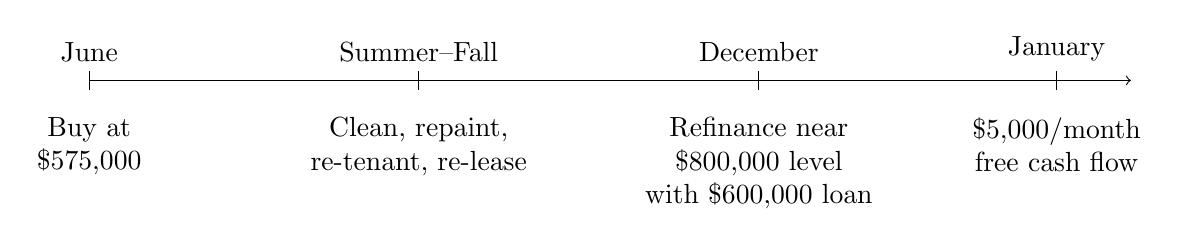
\begin{tikzpicture}[x=2.7cm,y=1cm]
\draw[->] (0,0) -- (4.9,0);
\foreach \x in {0,1.55,3.15,4.55}
  \draw (\x,0.12) -- (\x,-0.12);

\node[align=center,above] at (0,0.12) {June};
\node[align=center,below] at (0,-0.35) {Buy at\\\(\$575{,}000\)};

\node[align=center,above] at (1.55,0.12) {Summer--Fall};
\node[align=center,below] at (1.55,-0.35) {Clean, repaint,\\re-tenant, re-lease};

\node[align=center,above] at (3.15,0.12) {December};
\node[align=center,below] at (3.15,-0.35) {Refinance near\\\(\$800{,}000\) level\\with \(\$600{,}000\) loan};

\node[align=center,above] at (4.55,0.12) {January};
\node[align=center,below] at (4.55,-0.35) {\(\$5{,}000\)/month\\free cash flow};
\end{tikzpicture}
\caption{Transcript-based reconstruction of the first-property sequence. The drawing is an analytic aid; the underlying claims come from the narrated purchase-improve-refinance-cash-flow order.}
\end{figure}

\paragraph{Worked arithmetic.}
If we keep strictly to what the lecture gives, the internal logic runs as follows.
\begin{enumerate}
\item The acquisition is nearly all-in. The remaining bank balance is said to be \(\$50\).
\item Operational work improves the property quickly enough to support a higher refinance-related value level.
\item The refinance loan is \(\$600{,}000\), while the original purchase price was \(\$575{,}000\), so at the most basic level we have
\begin{equation}
L_1 - P_0 = \$600{,}000 - \$575{,}000 = \$25{,}000.
\end{equation}
\item That difference alone does \emph{not} prove that every dollar of closing cost and improvement cost has been recovered, because the lecture does not give us a full capital stack.
\item It does, however, show why Napola can plausibly say that the property was improved enough to refinance, pull money back out, and leave him with recurring cash flow.
\item If we simply annualize the reported monthly figure, then the narrated rate of cash generation is
\begin{equation}
CF_{\text{yr}} = 12\,CF_{\text{mo}} = 12 \times \$5{,}000 = \$60{,}000/\text{year}.
\end{equation}
This annualization is only a clean restatement of the monthly claim; it is not a full pro forma.
\end{enumerate}

The force of the story lies in the change of economic form. At the start, income depends on trades. By the end, the speaker is describing an asset that has returned capital and begun paying him every month. That is why this passage occupies the center of the lecture: it is the first place where philosophy becomes arithmetic.

\section{Books, Time Horizons, and the Three Takeaways}

After the first-property case, the lecture expands again. We move from one transaction back to the wider intellectual habits that make such a transaction thinkable. Napola credits Tony Robbins as an early force, especially the claim that people overestimate what they can do in one year and underestimate what they can do in five. The interview does not formalize that sentence, but it uses it to restore a long horizon after the compression of the case study.

He then shifts from one author to reading in general. This is not filler. It is another form of commercial leverage. The lecture makes the arithmetic of reading explicit enough that we may as well write it down. If one book distills roughly \(25\) to \(30\) years of experience, and even a slow reader gets through one book a month, then the yearly intake of experience is on the order of
\begin{equation}
12\ \text{books/year} \times (25\text{--}30\ \text{years/book})
= 300\text{--}360\ \text{years of experience/year}.
\end{equation}
That equation is only a restatement of the speaker's own rough reasoning, but it reveals something important about the lecture. Mentors and books play analogous roles. Both compress time.

The reading passage then turns into a recap structure when the interviewer asks for the top three takeaways from Napola's own book. The first is the strongest thesis in the interview: whatever their original industry, the richest people on the planet continue to allocate into real estate.

\begin{figure}[h]
\centering

\includegraphics[width=0.82\textwidth]{lecture_110_figure_03.png}
\caption{On-screen emphasis for the lecture's central capital-allocation claim.}
\end{figure}

This is not a mathematical identity. It is a capital-allocation thesis. But it grounds the rest of the argument. Real estate is not presented as an eccentric niche. It is presented as a terminal asset class, a place where successful people in many sectors eventually want to store and extend wealth.

The second takeaway is more personal and therefore more useful. Different property types fit different lives. A dentist with no time for active management should not pretend to be a value-add operator. A person with time and appetite for direct involvement may do well precisely there. The notes should preserve this fit between property type and operator type. The lecture does not want us to confuse the generic attractiveness of real estate with the claim that every asset structure suits every life.

The third takeaway is pedagogical: commercial property is easier than people think, especially if one begins with something one can manage directly. That ease is not the ease of push-button wealth. It is the ease that comes after the business stops looking mystical.

At this point the lecture folds back to retirement security. Napola's claim is modest in form but large in implication:
\begin{equation}
T_{\text{payoff}} \approx 20\text{--}25\ \text{years}
\;\Rightarrow\;
\text{one paid-off property can become a retirement base.}
\end{equation}
The claim is heuristic, not guaranteed. One correctly bought and patiently held property may not make a person rich, but it can fundamentally alter later-life vulnerability. This is exactly the sort of sentence the lecture wants us to carry forward.

\section{The Entry Barrier Inverted}

The interview now raises the cleanest obstacle in the whole discussion. Many people think real estate begins only after a large pile of personal money has already been accumulated. Napola answers by reversing the scarcity claim.

\subsection{Question \& Answer}

\paragraph{Question.}
How can someone with little money, little credit, and no obvious balance-sheet strength still get into real estate?

\paragraph{Answer.}
The lecture's answer is to move our attention away from money and toward deal quality. Napola invokes Aventura Mall as a local example. If the mall is worth roughly \$3 billion, and someone offered it tomorrow for \$1 billion, money would not be the hard part:
\begin{align}
V_{\text{mall}} &\approx \$3\times 10^9, &
P_{\text{hyp}} &= \$1\times 10^9.
\end{align}
The point is not that such a transaction is likely. The point is that the financing problem changes character when the opportunity is extraordinary. In that sense the lecture's governing inversion is
\begin{equation}
D_{\text{good}} \Rightarrow K_{\text{outside}}\ \text{is easier to source.}
\end{equation}
Equally important is the converse warning:
\begin{equation}
K_{\text{own}}\ \text{small} \not\Rightarrow D_{\text{good}}\ \text{impossible.}
\end{equation}

So the interview relocates the bottleneck. The beginner's error is to think that the scarce object is money. Napola insists that the scarce object is a genuinely good deal. There is, in his phrase, a line of people a hundred miles long who want to put money into strong opportunities but cannot find them.

\begin{figure}[h]
\centering
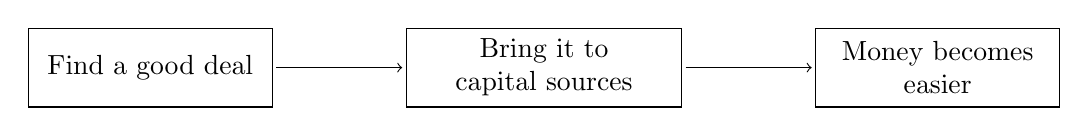
\begin{tikzpicture}[x=1cm,y=1cm]
\node[draw,align=center,minimum width=3.1cm,minimum height=1cm] (a) at (0,0) {Find a good deal};
\node[draw,align=center,minimum width=3.5cm,minimum height=1cm] (b) at (5,0) {Bring it to\\capital sources};
\node[draw,align=center,minimum width=3.1cm,minimum height=1cm] (c) at (10,0) {Money becomes\\easier};
\draw[->] (1.6,0) -- (3.2,0);
\draw[->] (6.8,0) -- (8.4,0);
\end{tikzpicture}
\caption{Transcript-based schematic of the lecture's inversion: the hard step is locating the deal; capital is downstream.}
\end{figure}

The logical sequence is therefore:
\begin{enumerate}
\item stop defining the barrier as personal cash alone,
\item learn to recognize an opportunity with genuine margin in it,
\item bring that opportunity to people who know how to finance strong deals,
\item use the deal itself as the persuasive object.
\end{enumerate}

That is one of the cleanest conceptual resolutions in the chapter, and it deserves to stand on the page as a `Question \& Answer' rather than being diluted into generic encouragement.

\section{Local Edge, Contrarian Timing, and the Right Why}

Once entry is reframed, the lecture turns to the next problem: how does one compete once one is in the business? Napola's answer is not scale for its own sake. It is control and proximity.

He says the firm's properties are kept within roughly \(250\) to \(300\) miles of the office:
\begin{align}
R &\approx 250\text{--}300\ \text{miles}, &
A_{\text{deal}} &= 165{,}000\ \text{sq ft}, \\
P_{\text{deal}} &= \$25{,}000{,}000. &&
\end{align}
The radius \(R\) is itself a piece of strategy. If we can wake up, drive to the property, inspect it, understand it, address an issue, and return home by dinner, we possess a kind of edge that a scattered national buyer may not. That edge is amplified by doing the work in-house: leasing, accounting, and property management sit close enough together that information circulates quickly. Tenants at one property can help identify tenants for another. One manager's knowledge can inform another manager's vacancy problem. The lecture treats these synergies as concrete, not rhetorical.

The \$25 million acquisition described later in the interview is then presented as the larger-scale version of the same operating intelligence. The property, never formally marketed, had been built by a father and son over roughly ten years and passed into a more complicated heirship structure. Once again, the transaction emerges from a readable human and institutional situation, not from blind market surfing.

The lecture then adds a contrarian rule. We are told to go against the grain. If everyone fears office, that fear may itself be a source of pricing distortion. If everyone says retail is dead, one ought to inspect whether that slogan has outrun reality. If the herd rushes into whatever is fashionable now, that may be the moment for caution rather than imitation. The interview does not formalize this with a market model, but the decision rule is sharp enough:
\begin{enumerate}
\item when fear is indiscriminate, look more closely rather than less,
\item when enthusiasm is indiscriminate, tighten standards rather than loosen them,
\item buy what fits our knowledge and only when the deal is still good.
\end{enumerate}

The closing movement of the lecture is inward again. Wealth is no longer defined by what can be displayed. It is defined by the right why. If the motive is a fancy car or a fancy dinner, Napola says the project will not hold. If the motive is financial freedom, support for parents, education for children, and the end of month-to-month fear, then persistence becomes more believable.

\subsection{Question \& Answer}

\paragraph{Question.}
What happens if the bank account goes to zero tomorrow? How does one begin again?

\paragraph{Answer.}
The lecture resolves this by distinguishing money from accumulated operating capital. A cash balance can vanish without erasing knowledge, contacts, reputation, or pattern recognition. In that sense,
\begin{equation}
B = 0 \not\Rightarrow
\bigl(
\text{knowledge}=0,\;
\text{contacts}=0,\;
\text{reputation}=0
\bigr).
\end{equation}
This is the final inversion of the chapter. A person who has already learned how deals work is not in the same position as a novice, even if the bank balance happens to be identical on one particular day. That is why Napola says he would return to real estate immediately if forced to rebuild. The assets that matter most at that stage are no longer merely monetary.

\section{Summary}

We can now see the architecture of the lecture more clearly. It begins with scale, but it does not stay there. It moves to mentorship in order to show how time can be compressed. It moves to anti-comparison discipline in order to clear the emotional ground for real risk. It then gives us its central arithmetic: buy, improve, refinance, recover, and hold for recurring cash flow. From there it broadens into doctrine. Real estate is where major pools of capital ultimately want to sit; one paid-off asset can change the shape of retirement; the true scarcity is the good deal rather than the money; local control is a real edge; and resilience at the end depends less on the current bank balance than on accumulated commercial intelligence. The interview remains conversational throughout, but its logic is tight: durable wealth is built by changing the form of income, the structure of ownership, and the quality of one's operating judgment.